\section{Wähle ein Sprite aus und bewege es in 4 Richtungen}
\subsection{Aufgabe}
Scratch Exercise 1: .

Das Scratch Programm wurde am MIT entwickelt, um jungen Schülern die Programmierung und die Multimedia Kommunikation beizubringen. 

Die Programmierung erfolgt durch ein visuelles System, die Kacheln oder Tiles. Diesen können Befehle zugeordnet werden und durch das zusammenlegen der Kacheln entstehen die Programme. Die Programme steuern Figuren und Objekte innerhalb des Spiels.


\subsection{Die Scratch Oberfläche}
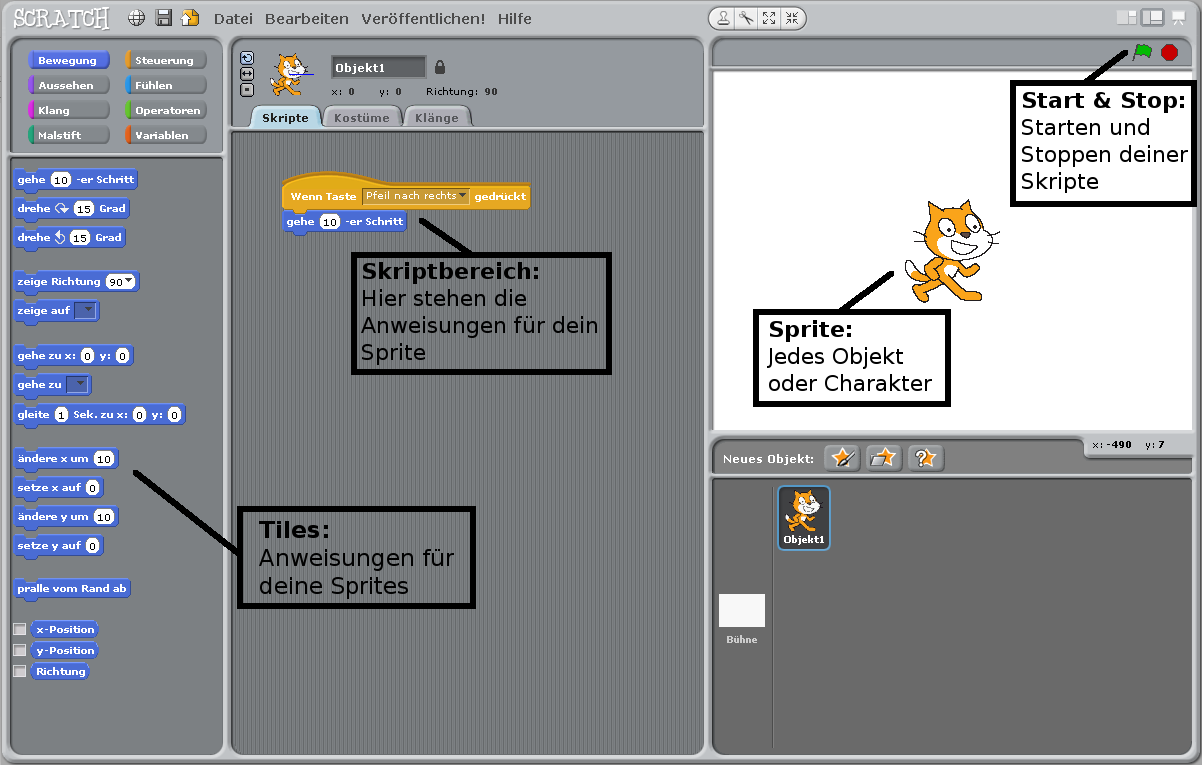
\includegraphics[width=\textwidth]{images/example1_overview.png}

\subsubsection{Wähle einen Sprite}

Ein Sprite ist eine Figur oder ein Objekt in deinem Spiel. Die Sprites können sich bewegen oder still stehen. Wir wählen eine Sprite-Figur und lassen sie über deinen Bildschirm laufen.
\begin{enumerate}
\item Öffne Scratch
\item Öffne den Ordner in den Scratch installiert wurde.
\item Klicke doppelt auf das Scratch-Icon.
\item Nun siehst du den Startbildschirm.
\item Klicke auf den Reiter \textit{Kostüme}
\item Klicke auf \textit{Importieren}
\item Wähle den Ordner (Animals (dt. Tiere), People (dt. Menschen), Things (dt. Dinge)
\item Wähle einen  Sprite! (Doppelklick)
\end{enumerate}

\subsubsection{Bewege deinen Sprite in 4 Richtungen (Rechts, Links, Hoch, Runter)}

Sprites können eigentlich nichts von sich aus. Eine Sprite-Aktion kommt direkt aus einem Skript aus dem Skript-Editor. Diese Skripte sind die Anweisungen für genau das was ein Sprite tun soll.
Du ziehst die Anweisung mit deiner Maus aus der linken Kachelspalte in die Skriptspalte. Die Kacheln passen wie Puzzleteile ineinander und bilden eine Anweisung.


\begin{enumerate}
\item Klicke auf den Sprite-Reiter
\item Wenn du dein Sprite nach rechts bewegen willst, klicke auf den Steuerung-Button.
\item Klicke mit der linken Maustaste auf eine Anweisung und halte die Taste gedrückt. Ziehe nun den Befehl
 \textit{Wenn Taste Leertaste gedrückt} nach rechts in die Skriptfläche. 
\item Klicke auf das Wort \textit{Leertaste} und wähle \textit{Pfeil nach rechts} aus.  (Wir bewegen den Sprite nach rechts)
\item Klicke auf den Bewegung-Button, oben links, und ziehe die Kachel “zeige Richtung 90” in das Skript-Fenster.
\item Verbinde \textit{Wenn Taste Pfeil nach Rechts} mit \textit{zeige Richtung 90}
\item Klicke auf das \textit{gehe 10-er Schritte} und ziehe es in das Skript-Fenster 
\item Verbinde die Kacheln wie auf dem Bild. 
\item Klicke den Pfeil-Button deiner Tastatur und deine Figur bewegt sich.
\item Bewegen wir unser Sprite nach links: Drag Ziehe den \textit{wenn Leertaste gedrückt}-Button in das Skriptfenster .
\item Ändere \textit{Leertaste} zu \textit{Pfeil nach links gedrückt}
\item Ziehe \textit{zeige Richtung 90} aus dem Bewegungsfenster in das Skript-Fenster.
\item Ändere die 90 zu -90.
\item Ziehe die \textit{gehe 10er Schritte}-Kachel in das Skriptfenster und verbinde es mit der vorherigen Kachel.
( Wenn es bei dir aussieht wie auf dem Bild, ist alles korrekt!)
\item Jetzt sollte auch dein linker Pfeil auf der Tastatur funktionieren! Klicke auf den Doppelpfeil, damit sich die Figur auch in die richtige Laufrichtung dreht. 
\item Lass deine Figur sich nach unten bewegen: Ziehe und verbinde dazu folgende Kacheln:
\subitem \textit{Wenn Leertaste gedrückt}
\subitem \textit{Zeige Richtung 90}
\subitem \textit{gehe 10 Schritte}
\end{enumerate}

\subsubsection{Ändere die Richtung in \textit{unten 180}}
Ändere \textit{Leertaste} zu \textit{Pfeil nach unten}
Jetzt funktioniert auch der Pfeil nach unten auf deiner Tastatur. 
\begin{enumerate}

\item Lass deine Figur sich nach oben bewegen: Ziehe und verbinde dazu folgende Kacheln:
\subitem \textit{Wenn Leertaste gedrückt}
\subitem \textit{Zeige Richtung 90}
\subitem \textit{gehe 10 Schritte}
\item Setze die Richtung auf  \textit{0 - Oben}:
\end{enumerate}
Ändere \textit{Leertaste} zu \textit{Pfeil nach oben}

\begin{enumerate}
\item Jetzt bewegt sich dein Sprite in alle 4 Richtungen. Überprüfe es !
\item Gib deinem Sprite einen Namen.
\item Speichere dein Programm
\end{enumerate}